\documentclass{article}
\usepackage{graphicx}
\usepackage{hyperref}
\usepackage[svgnames]{xcolor}
\usepackage{listings}

% some adjustments for the lstlisting environment used to typeset code
\lstset{backgroundcolor=\color{LightSteelBlue!60},
  frame=trbl,
  rulecolor=\color{black!30},
  xrightmargin=7pt}

\begin{document}
\title{Multicast Routing in Linux}
\author{Ang Way Chuang \\
\small{\href{mailto:wcang@sfc.wide.ad.jp}{wcang@sfc.wide.ad.jp}}}
\date{\today}
\maketitle
\section{Foreword}
This is part of an ongoing effort to understand how multicast forwarding works
and implementation of multicast routing within a routing daemon on Linux (UNIX)
system. Those who want to look for guide to write multicast application should
look elsewhere. As my understanding on multicast routing is quite limited,
errors are to be expected and the document will remain incomplete and
disorganized until I have a better understanding on the subject. I would like to
thank Afumado Basuki for his encouragement and his eargerness to share his
knowledge. 

There are a lot of online references on PIM multicast routing and this is just
one of them. This document tries to address that gap. This document refers to
the implementation of Linux kernel version 3.1.0, but the discussion should
apply to older and newer kernels that implements multicast routing. Due to time
limit, this document shall limit itself to the discussion of IPv6.

\section{Multicast Forwarding}
\begin{figure}[h]
  \begin{center}
    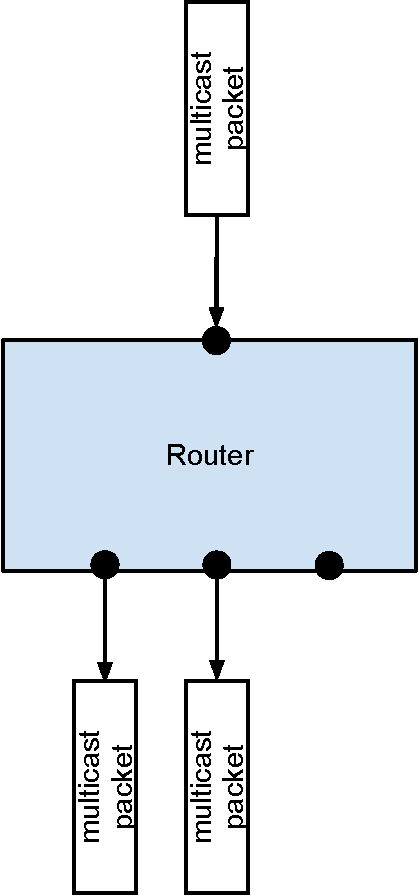
\includegraphics[width=0.3\textwidth]{mcast-forward}
    \caption{Router duplicates and send out multicast packet to the
    outgoing interfaces that have active listeners of multicast group}
    \label{fig:mcast-forward}
  \end{center}
\end{figure}

As shown in Figure \ref{fig:mcast-forward}, unlike unicast forwarding, when a
multicast packet is received by a router, the packet may be forwarded to
multiple outgoing interfaces. While, it is the job of the kernel to duplicate
the packet and forward the multicast packet to all the relevant outgoing
interfaces based on Multicast Forwarding Cache (MFC), the kernel does not know
which interfaces to forward the multicast packet. What the kernel provides is an
interface to install an MFC entry. Multicast routing daemon (typically running
PIM protocol) will learn about the active listeners of the multicast stream and
decide which outgoing interfaces the multicast packet should be forwarded to.
Multicast routing daemon should then install an appropriate MFC entry into
kernel accordingly.

To make a parallel comparison with unicast forwarding, one could say while it is
the job of the kernel to forward a unicast packet based on routing table, the
kernel does not know every possible routes. What the kernel provides is an
interface to install (unicast) route entries into the routing table. It is the
job of unicast routing daemon (running dynamic routing protocol) to learn the
network topology and install route entries accordingly.

The difference between a route entry and an MFC entry is that a route entry
typically consists of a network with its prefix and a single outgoing interface,
while an MFC entry consists of the following tuple:
\begin{itemize}
  \item source address - source (S) address of multicast packet
  \item group address - group (G) address of multicast packet
  \item incoming interface - the network interface where the multicast packet
  belonging to the (S,G) should be received. This information will be used for
  RPF checking within the kernel (\texttt{ip6\_mr\_forward}). RPF checking is
  done solely based on MFC entry. At first, it seems counter-intuitive to have
  this additional parameter as the kernel can perform RPF checking based on its
  routing table.  While the kernel has the required information to perform RPF
  checking based on unicast Forwarding Information Base (FIB, or in other word,
  routing table), it doesn't know about the Multicast Forwarding Information
  Base (MFIB) because there is no corresponding FIB for multicast in the kernel.
  Only the multicast routing daemon has the information on MFIB. For typical
  deployment, most of the entries of MFIB corresponds to FIB as MFIB is mostly
  constructed from FIB. However, there are situation where it may differ. Apart
  from that, the incoming interface for a multicast stream may be different when
  the stream is delivered through Rendezvous Point Tree (RPT) and Shortest Path
  Tree (SPT). Therefore, the routing daemon may need to modify this parameter when
  it switches the multicast stream from RPT to SPT.
  \item list of outgoing interfaces - the list of network interfaces where the
  multicast packet belonging to (S,G) should be forwarded 
\end{itemize}

User space routing daemon can manipulate MFC using \texttt{mf6cctl\{\}}
(\texttt{<linux/mroute6.h>}). Within the kernel, an MFC entry is represented by
\texttt{mfc6\_cache\{\}} (\texttt{include/linux/mroute6.h}).

The following subsections will highlight the multicast packet traversal process
for 2 MFC states:

\begin{itemize}
  \item unresolved (queued) state - Unresolved state only happens when there is
  no pre-installed (by routing daemon) MFC entry when a (S,G) multicast packet
  is received. In this case, the kernel will create an unresolved (or called
  queued) MFC entry for the multicast packet. In this state, multicast packet
  cannot be forwarded because it doesn't know the outgoing interfaces.
  \item resolved state - In this state, the MFC entry is used to assist with the
    multicast forwarding. Most literature refers to this state when MFC is
    mentioned because unresolved MFC entry cannot be used to performed multicast
    forwarding.
\end{itemize}

 
\subsection{MFC States}
\label{sec:mfc-states}
\begin{figure}[h]
  \begin{center}
    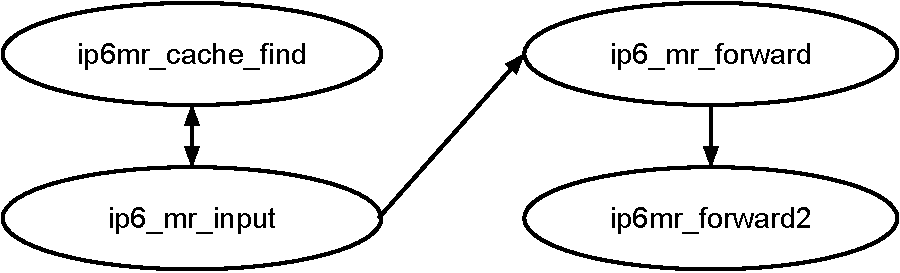
\includegraphics[width=\textwidth]{mcast-mfc}
    \caption{Interaction between kernel and user space routing daemon on the
    occassion of unresolved and resolved MFC states}
    \label{fig:mcast-unresolved}
  \end{center}
\end{figure}

Figure \ref{fig:mcast-unresolved} is the simplified interaction of kernel and
user space routing daemon in the process of forwarding multicast packet. Let's
begin with the resolved state as it is the simpler one. The processing of a
multicast packet begins with \texttt{ip6\_mr\_input}. \texttt{ip6\_mr\_input}
calls \texttt{ip6mr\_cache\_find} to lookup for a matching MFC entry based on
the source and group addresses of the multicast packet. All resolved MFC entries
are stored in \texttt{mfc6\_cache\_array} list of \texttt{mr6\_table}.  Barring
the usage of namespace, typical deployment will only have single
\texttt{mr6\_table} to manage multicast forwarding. In the case of resolved
state, \texttt{mfc6\_cache\_find} will return a matching MFC entry. In which
case, \texttt{ip6\_mr\_input} will pass the packet directly to
\texttt{ip6\_mr\_forward}. For each outgoing interface that has active listener,
\texttt{ip6mr\_forward2} will be called to forward the packet to the interface.
The current code in \texttt{ip6\_mr\_forward} forwards to multicast packet if the
hop limit of the multicast packet is greater than TTL threshold of the outgoing
interface. This implementation is buggy. TTL threshold is only relevant for
IPv4. Further explanation will be given in section
\label{sec:multicast-interface}.

In the case of unresolved state, there will not be any matching MFC entry. The
packet will be passed to \texttt{ip6mr\_cache\_unresolved}.
\texttt{ip6mr\_cache\_unresolved} will create an unresolved MFC entry for the
packet if there is no prior unresolved MFC entry for this packet and enqueue the
packet into the MFC entry. All unresolved MFC entries are enqueued within the
\texttt{mfc6\_unres\_queue} list of \texttt{mr6\_table}.


\texttt{ip6mr\_cache\_unresolved} will call \texttt{ip6mr\_cache\_report}.
\texttt{ip6mr\_cache\_report} will create a packet to inform routing daemon of
the unresolved cache event using multicast socket. The packet is an IPv6 packet.
The format of the packet is shown in Figure \ref{fig:mcast-upcall}:

\begin{figure}[h]
  \begin{center}
    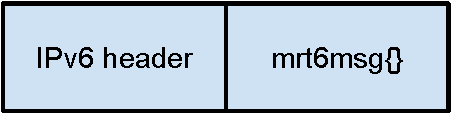
\includegraphics[width=0.4\textwidth]{mcast-upcall}
    \caption{Packet format of IPv6 multicast upcall}
    \label{fig:mcast-upcall}
  \end{center}
\end{figure}

\texttt{im6\_mif}, \texttt{im6\_src} and \texttt{im6\_dst} of
\texttt{mrt6msg\{\}} contains sufficient information for routing daemon to
determine the list of outgoing interfaces and install a corresponding MFC using
\texttt{setsockopt(fd, IPROTO\_IPV6, MRT6\_ADD\_MFC, \ldots)}. Corresponding to
that, kernel's \texttt{ip\_mroute\_setsockopt} will call
\texttt{ip6mr\_mfc\_add} to add a new (resolved) MFC entry and remove the
corresponding unresolved MFC entry from the list. \texttt{ip6mr\_cache\_resolve}
will forward all the queued multicast packets in the unresolved MFC entry to the
list of outgoing interfaces found in the newly added resolved MFC entry. All MFC
entries installed by the routing daemon (resolved) and kernel (unresolved) will
be listed in \texttt{/proc/net/ip6\_mr\_cache} like the following example:

\begin{lstlisting}
cat /proc/net/ip6_mr_cache
Group      Origin      Iif  Pkts Bytes  Wrong  Oifs
ff3e::1234 5050::2     3    0    0      0      4:1 5:1
ff3e::beac 2001:d30:101:2:6666:6666::1 -1         0        0        0

\end{lstlisting}

The output format of \texttt{/proc/net/ip6\_mr\_cache} is as such:
\begin{itemize}
  \item \texttt{Origin} is the source address.
  \item \texttt{Group} is the multicast group address. 
  \item \texttt{Iif} is the index of incoming interface. The meaning of the
    index will be explained in section \ref{sec:multicast-interface}. Unresolved
    MFC entry will have value of -1 of the index.
  \item \texttt{Pkts} and \texttt{Bytes} are the number of multicast packets
    forwarded and the number of bytes for these packets.
  \item \texttt{Wrong} is number of packets arriving at the wrong interface.
    This typically happens when there are multiple PIM routers on the same link
    forwarding for the (S,G).
  \item \texttt{Oifs} is the list of index of outgoing interfaces. In the
    example given above, multicast interfaces with index of 4 and 5 are used to
    forward the multicast packets. The number after the ``:'' delimiter is the
    TTL threshold. Do note that the value given by this field is incorrect due
    to a bug. However, the use of TTL threshold is not encouraged. Further
    explanation will be given in section \ref{sec:multicast-interface}.
\end{itemize}

If there is no active listener for a (S,G) multicast stream, the routing daemon
will not install any MFC entry even though it receives an upcall from the
kernel. The packets queued within unresolved MFC entry will be garbage collected
after its timer expires.

It can be said that most MFC entries will begin with unresolved state (and then
later be replaced by resolved MFC entries) because the router has no way to know
in advanced when a source is going to send multicast packet to a particular
group. Even though the routing daemon is capable of determining the list of
outgoing interfaces for a multicast packet belonging to any group, it is not
feasible to install a MFC entries for every possible sources for every possible
groups. There are exceptions to this behaviour. For Source Specific Multicast
(SSM) or cases where the source and group are known in advanced (e.g.  PIM
Join(S,G) or MLD(S,G)), the routing daemon may install a corresponding MFC entry
in advance thus avoiding the unresolved state altogether.

\section{Multicast Interface}
\label{sec:multicast-interface}
The need to have a dedicated API to enable multicast forwarding on an interface 
is not very obvious. To enable multicast forwarding on an interface,
\texttt{setsockopt(2)} should be called \texttt{MRT6\_ADD\_MIF} command. The data
structure \texttt{mif6ctl\{\}} should be passed to the kernel for that system
call. 

Let's look at the definition of \texttt{mif6ctl\{\}} from
\texttt{<linux/mroute6.h>}:

\begin{lstlisting}[basicstyle=\footnotesize]
/*
 *      Passed by mrouted for an MRT_ADD_MIF - again we use the
 *      mrouted 3.6 structures for compatibility
 */

struct mif6ctl {
  mifi_t  mif6c_mifi;           /* Index of MIF */
  unsigned char mif6c_flags;    /* MIFF_ flags */
  unsigned char vifc_threshold; /* ttl limit */
  __u16    mif6c_pifi;          /* the index of the physical IF */
  unsigned int vifc_rate_limit; /* Rate limiter values (NI) */
};
\end{lstlisting}

Of the five fields, only three fields should be used. This struct is not used by 
\texttt{mrouted} as the comment would have us believe because \texttt{mrouted}
only supports DVMRP which is supposed to work on IPv4 only. This data structure
may be a poorly thought-out copy of its IPv4 counterpart. The explanation of
each individual field as such:

\begin{itemize}
  \item \texttt{mif6c\_mifi} - This is the multicast interface index.  This
    value should be assigned by the user of the API in a manner that ensures
    each multicast interface is given the unique value. It appears that valid
    index should be in the range from 0 to \texttt{MAXMIFS} - 1. In Linux,
    \texttt{MAXMIFS} is 32. In FreeBSD, \texttt{MAXMIFS} is 64. Thus, multicast
    forwarding can only be enabled on at most 32 interfaces in Linux.
  \item \texttt{mif6c\_flags} - The only valid flag at this moment is
    \texttt{MIFF\_REGISTER}. When this flag is set, a virtual interface will be
    created to handle PIM REGISTER tunnel.
  \item \texttt{vifc\_threshold} - This is supposed to be TTL threshold value
    discussed in the previous section. Using this field is not compatible with
    FreeBSD and current implementation of TTL threshold is buggy. The purpose of
    TTL threshold is to limit the flow of multicast traffic to a certain segment
    of network by setting high threshold value. A multicast packet is forwarded
    through an interface only if its TTL (hop limit) is greater than the TTL
    threshold of the interface. Another purpose of TTL threshold is to mitigate
    the problem of count-to-infinity in DVMRP. This is not an issue for IPv6.
    Besides, it is better to use administrative scoping of IPv6 multicast
    address (RFC4291) to limit the flow of multicast packets. In short, this
    field should not be used.
  \item \texttt{mif6c\_pifi} - The is the index of ``physical'' interface. This
    is the index returned by \texttt{if\_nametoindex(3)}. Special treatment is
    given for PIM REGISTER interface because PIM REGISTER doesn't have a
    corresponding network interface before \texttt{MRT\_ADD\_MIF} is called.
    When \texttt{MIFF\_REGISTER} is set on \texttt{mif6c\_flags}, the value of
    this field is ignored by the kernel.
  \item \texttt{vifc\_rate\_limit} - The functionality for this field is not
    implemented and FreeBSD's \texttt{mif6ctl} does not have this field either.
    This field should not be used.
\end{itemize}

Without enabling multicast forwarding on an interface using
\texttt{MRT6\_ADD\_MIF}, multicast packet cannot be forwarded through the
interface because adding a new MFC entry requires multicast interface index.
There seems to be no good explanation for the need of another set of index just
for multicast forwarding and thereby limiting the number of multicast interface
to \texttt{MAXMIFS}. By looking at the kernel implementation of multicast
interface, the \texttt{mif6c\_mifi} is just an index into array table
(\texttt{mr6\_table\{\}}) for fast reference. The same can be said for FreeBSD
9.0 kernel. Direct indexing into array table in the kernel is the only side
effect of implementation, it is believed that the main purpose of having a
separate index for multicast enabled interface is to assist the setting of oif
list (\texttt{mf6cc\_ifset} of \texttt{mf6cctl\{\}}).

It is in my humble opinion that a properly design API should not limit the
number of multicast forwarding enabled interface in this artificial manner. If
the API is designed properly, specifying \texttt{mif6c\_pifi} should be
sufficient for the kernel to enable multicast forwarding on a network interface.

Having said that, why is there a need to have an API to enable multicast
forwarding on an interface explicitly? Assuming that there is no such thing as
multicast interface index, isn't easier to have an API that lets the routing
daemon to enable multicast forwarding by simply adding new MFC directly without
calling \texttt{MRT6\_ADD\_MIF} first. Well, there is a good reason not to have
such kind of API. In order to install a new MFC entry, routing daemon needs to
know when an (S,G) is actively flowing (for the case PIM's shared tree traffic).
Routing daemon typically learns about this from the kernel upcall. However,
kernel upcall rely upon the caching of unresolved MFC state as explained in
section \ref{sec:mfc-states}. Only interfaces with multicast forwarding enabled
should have the caching of unresolved MFC state because enabling such mechanism
on all interfaces is a waste of resource.

To determine the interface with multicast forwarding, a user can look at
\texttt{/proc/net/ip6\_mr\_vif}. What follows is an example:
\begin{lstlisting}
# cat /proc/net/ip6_mr_vif
Interface      BytesIn  PktsIn  BytesOut PktsOut Flags
 3 eth1              0       0         0       0 00000
 4 eth2              0       0         0       0 00000
\end{lstlisting}

The \texttt{Interface} field basically consists of multicast interface index
(\texttt{mif6c\_mifi} and the name of the network interface, while the
\texttt{Flags} field reflects the value of \texttt{mif6c\_flags}. In addition
that, such information can be obtained through sysctl. For example:

\begin{lstlisting}
# sysctl net.ipv6.conf.eth1.mc_forwarding
net.ipv6.conf.eth1.mc_forwarding = 1
\end{lstlisting}

In this example, multicast forwarding is enabled on eth1. Do note that
\texttt{net.ipv6.conf.\textit{iface}.mc\_forwarding} is a read-only file. One
cannot enable nor disable multicast forwarding by toggling this sysctl file.

\section{References}
IPv6 Advanced Protocol Implementations

RFC 4601

RFC 4291 http://tools.ietf.org/html/rfc4291

http://manpages.ubuntu.com/manpages/hardy/man4/multicast.4.html

http://manpages.ubuntu.com/manpages/hardy/man4/pim.4.html

Multicast over TCP/IP HOWTO http://tldp.org/HOWTO/Multicast-HOWTO.html
\end{document}
